% 
% 
% 
% 
% 
% 
% 



\tikzset{every picture/.style={line width=0.75pt}} %set default line width to 0.75pt        

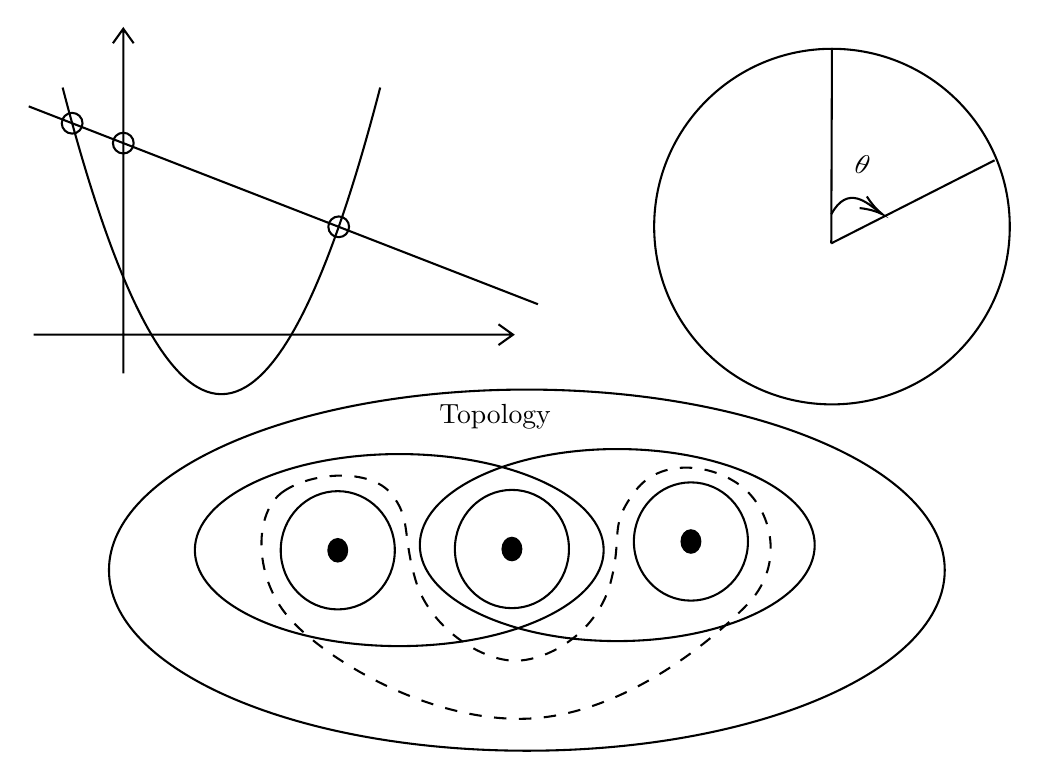
\begin{tikzpicture}[x=0.75pt,y=0.75pt,yscale=-1,xscale=1]
    %uncomment if require: \path (0,365); %set diagram left start at 0, and has height of 365

    %Shape: Axis 2D [id:dp3330650107827038] 
    \draw  (52.67,153.74) -- (283.67,153.74)(95.9,6.33) -- (95.9,172.41) (276.67,148.74) -- (283.67,153.74) -- (276.67,158.74) (90.9,13.33) -- (95.9,6.33) -- (100.9,13.33)  ;
    %Shape: Parabola [id:dp6747224874888704] 
    \draw   (66.67,34.67) .. controls (117.67,231.65) and (168.67,231.65) .. (219.67,34.67) ;
    %Straight Lines [id:da4045208158970277] 
    \draw    (50.33,43.74) -- (295.67,139.07) ;
    %Shape: Circle [id:dp9495260244967654] 
    \draw   (351.67,101.67) .. controls (351.67,54.35) and (390.02,16) .. (437.33,16) .. controls (484.65,16) and (523,54.35) .. (523,101.67) .. controls (523,148.98) and (484.65,187.33) .. (437.33,187.33) .. controls (390.02,187.33) and (351.67,148.98) .. (351.67,101.67) -- cycle ;
    %Straight Lines [id:da6440917457226727] 
    \draw    (437.33,16) -- (437,109.74) ;
    %Straight Lines [id:da2506243181764847] 
    \draw    (515.67,69.74) -- (437,109.74) ;
    %Curve Lines [id:da36631824919286937] 
    \draw    (437,95.74) .. controls (444.89,81.18) and (454.43,90.36) .. (460.1,94.64) ;
    \draw [shift={(461.67,95.74)}, rotate = 212.01] [color={rgb, 255:red, 0; green, 0; blue, 0 }  ][line width=0.75]    (10.93,-3.29) .. controls (6.95,-1.4) and (3.31,-0.3) .. (0,0) .. controls (3.31,0.3) and (6.95,1.4) .. (10.93,3.29)   ;
    %Shape: Ellipse [id:dp9329672718104849] 
    \draw   (89,267.19) .. controls (89,219.14) and (179.14,180.19) .. (290.33,180.19) .. controls (401.53,180.19) and (491.67,219.14) .. (491.67,267.19) .. controls (491.67,315.24) and (401.53,354.19) .. (290.33,354.19) .. controls (179.14,354.19) and (89,315.24) .. (89,267.19) -- cycle ;
    %Shape: Ellipse [id:dp9998724111128214] 
    \draw   (130.37,257.52) .. controls (130.37,231.97) and (174.47,211.26) .. (228.86,211.26) .. controls (283.25,211.26) and (327.34,231.97) .. (327.34,257.52) .. controls (327.34,283.08) and (283.25,303.79) .. (228.86,303.79) .. controls (174.47,303.79) and (130.37,283.08) .. (130.37,257.52) -- cycle ;
    %Shape: Ellipse [id:dp6415322670258081] 
    \draw   (238.76,255.11) .. controls (238.76,229.56) and (281.35,208.84) .. (333.89,208.84) .. controls (386.43,208.84) and (429.02,229.56) .. (429.02,255.11) .. controls (429.02,280.66) and (386.43,301.37) .. (333.89,301.37) .. controls (281.35,301.37) and (238.76,280.66) .. (238.76,255.11) -- cycle ;
    %Shape: Ellipse [id:dp6607583700307356] 
    \draw   (171.75,257.62) .. controls (171.75,241.88) and (184.05,229.13) .. (199.23,229.13) .. controls (214.4,229.13) and (226.71,241.88) .. (226.71,257.62) .. controls (226.71,273.35) and (214.4,286.11) .. (199.23,286.11) .. controls (184.05,286.11) and (171.75,273.35) .. (171.75,257.62) -- cycle ;
    %Shape: Ellipse [id:dp7853319365959068] 
    \draw   (255.66,257.01) .. controls (255.66,241.28) and (267.96,228.52) .. (283.14,228.52) .. controls (298.32,228.52) and (310.62,241.28) .. (310.62,257.01) .. controls (310.62,272.75) and (298.32,285.5) .. (283.14,285.5) .. controls (267.96,285.5) and (255.66,272.75) .. (255.66,257.01) -- cycle ;
    %Shape: Ellipse [id:dp5078229765284272] 
    \draw   (341.9,253.39) .. controls (341.9,237.65) and (354.21,224.9) .. (369.38,224.9) .. controls (384.56,224.9) and (396.86,237.65) .. (396.86,253.39) .. controls (396.86,269.12) and (384.56,281.88) .. (369.38,281.88) .. controls (354.21,281.88) and (341.9,269.12) .. (341.9,253.39) -- cycle ;
    %Shape: Ellipse [id:dp47882141993434524] 
    \draw  [fill={rgb, 255:red, 0; green, 0; blue, 0 }  ,fill opacity=1 ] (364.85,253.39) .. controls (364.85,250.4) and (366.88,247.97) .. (369.38,247.97) .. controls (371.89,247.97) and (373.92,250.4) .. (373.92,253.39) .. controls (373.92,256.38) and (371.89,258.81) .. (369.38,258.81) .. controls (366.88,258.81) and (364.85,256.38) .. (364.85,253.39) -- cycle ;
    %Shape: Polygon Curved [id:ds8181656794178567] 
    \draw  [dash pattern={on 4.5pt off 4.5pt}] (172.76,229.48) .. controls (186.67,219.68) and (214.76,218.15) .. (224.76,230.15) .. controls (234.76,242.15) and (230.1,249.48) .. (236.76,272.15) .. controls (243.43,294.82) and (268.63,311.28) .. (285.43,310.82) .. controls (302.23,310.35) and (324.76,296.15) .. (330.76,272.82) .. controls (336.76,249.48) and (329.43,246.15) .. (342.76,228.82) .. controls (356.1,211.48) and (384.1,216.82) .. (396.76,229.48) .. controls (409.43,242.15) and (413.43,266.15) .. (396.76,283.48) .. controls (380.1,300.82) and (335.47,338.48) .. (287.43,338.82) .. controls (239.39,339.16) and (189.43,307.48) .. (174.1,288.15) .. controls (158.76,268.82) and (158.86,239.29) .. (172.76,229.48) -- cycle ;
    %Shape: Ellipse [id:dp26952850031511955] 
    \draw  [fill={rgb, 255:red, 0; green, 0; blue, 0 }  ,fill opacity=1 ] (278.6,257.01) .. controls (278.6,254.02) and (280.63,251.59) .. (283.14,251.59) .. controls (285.65,251.59) and (287.68,254.02) .. (287.68,257.01) .. controls (287.68,260.01) and (285.65,262.43) .. (283.14,262.43) .. controls (280.63,262.43) and (278.6,260.01) .. (278.6,257.01) -- cycle ;
    %Shape: Ellipse [id:dp7070111192051278] 
    \draw  [fill={rgb, 255:red, 0; green, 0; blue, 0 }  ,fill opacity=1 ] (194.69,257.62) .. controls (194.69,254.62) and (196.72,252.2) .. (199.23,252.2) .. controls (201.73,252.2) and (203.76,254.62) .. (203.76,257.62) .. controls (203.76,260.61) and (201.73,263.04) .. (199.23,263.04) .. controls (196.72,263.04) and (194.69,260.61) .. (194.69,257.62) -- cycle ;

    % Text Node
    \draw (448.84,64.99) node [anchor=north west][inner sep=0.75pt]  [rotate=-12,xslant=0.03]  {$\theta $};
    % Text Node
    \draw (246.67,185.63) node [anchor=north west][inner sep=0.75pt]   [align=left] {Topology};

    \draw   (95.9, 61.45) circle [x radius= 5, y radius= 5]   ;
    \draw   (199.68, 101.77) circle [x radius= 5, y radius= 5]   ;
    \draw   (71.26, 51.87) circle [x radius= 5, y radius= 5]   ;
\end{tikzpicture}
% 
% 
% 
% 
% 